%\documentclass[12pt, letterpaper, titlepage]{article}
\documentclass[12pt, letterpaper]{article}

\usepackage{amsmath, amsfonts}
\usepackage{booktabs}
\usepackage{amsthm}
\usepackage{graphicx}
\usepackage[margin=1in]{geometry}
\usepackage{hyperref}
\usepackage{cleveref}
\hypersetup{colorlinks = true, linkcolor = blue, citecolor=blue, urlcolor = blue}
\usepackage{natbib}
\usepackage{float}
\usepackage{setspace}
\usepackage{pdfpages}
\usepackage{lineno}
\usepackage{mwe}
\usepackage{comment}
\linenumbers*[1]
% %% patches to make lineno work better with amsmath
\newcommand*\patchAmsMathEnvironmentForLineno[1]{%
 \expandafter\let\csname old#1\expandafter\endcsname\csname #1\endcsname
 \expandafter\let\csname oldend#1\expandafter\endcsname\csname end#1\endcsname
 \renewenvironment{#1}%
 {\linenomath\csname old#1\endcsname}%
 {\csname oldend#1\endcsname\endlinenomath}}%
\newcommand*\patchBothAmsMathEnvironmentsForLineno[1]{%
 \patchAmsMathEnvironmentForLineno{#1}%
 \patchAmsMathEnvironmentForLineno{#1*}}%

\AtBeginDocument{%
 \patchBothAmsMathEnvironmentsForLineno{equation}%
 \patchBothAmsMathEnvironmentsForLineno{align}%
 \patchBothAmsMathEnvironmentsForLineno{flalign}%
 \patchBothAmsMathEnvironmentsForLineno{alignat}%
 \patchBothAmsMathEnvironmentsForLineno{gather}%
 \patchBothAmsMathEnvironmentsForLineno{multline}%
}

% control floats
\renewcommand\floatpagefraction{.9}
\renewcommand\topfraction{.9}
\renewcommand\bottomfraction{.9}
\renewcommand\textfraction{.1}
\setcounter{totalnumber}{50}
\setcounter{topnumber}{50}
\setcounter{bottomnumber}{50}

\newcommand{\jy}[1]{\textcolor{blue}{JY: #1}}
\newcommand{\eds}[1]{\textcolor{red}{EDS: (#1)}}
\newcommand{\of}[1]{\textcolor{violet}{OF: #1}}

% NOTE: To produce blinded version, replace "0" with "1" below.
\newcommand{\blind}{0}

%\title{On Devon Allen's Disqualification at the 2022 World Track and Field
%Championships}
%
%\author{Owen Fiore\\
%%   \href{mailto:owen.fiore@uconn.edu}
%% {\nolinkurl{owen.fiore@uconn.edu}}\\
  %Elizabeth D. Schifano\\
  %Jun Yan\\[1ex]
  %Department of Statistics, University of Connecticut\\
%}
%\date{}

\begin{document}

\title{\bf Supplement to ``On Devon Allen's Disqualification at the 2022 World Track and Field Championships''}

\if0\blind
{
  \author{Owen Fiore, %\\
%   \href{mailto:owen.fiore@uconn.edu}
% {\nolinkurl{owen.fiore@uconn.edu}}\\
  Elizabeth D. Schifano, %\\
  Jun Yan\\[1ex]
  Department of Statistics, University of Connecticut\\
}
} \fi

\if1\blind
{
  \bigskip
  \bigskip
  \bigskip
  \author{Anonymous Authors}
  \bigskip
} \fi

\maketitle 

\section{Rank-Based Comparison with Pooled Men and Women Data}
As an alternative to the methods described in section 3.1 of the main paper, it
is possible to combine all men's and women's data for each of the three time
periods.  Thus we shrink our analyses from six to three, but each analysis
is roughly twice as big as previously.  For the 2019 versus 2022 comparison,
there were 258 reaction time observations from 65 athletes and the asymptotic
test result was a p value of $3.56 \cdot 10^{-8}$. For the 2022 national versus
internation comparison, there were 160 reaction time observations from 35
athletes and the asymptotic test result was a p value of $1.94 \cdot 10^{-7}$.
For the 2023 versus 2022 comparison, there were 343 reaction time observations
from 92 athletes and the asymptotic test result was a p value of
$4.99 \cdot 10^{-12}$.  These are all highly significant test results that show
substanial differences in average reaction time for athletes competing at
multiple championship level events.


\section{GAMLSS Results for Women Data}
We can repeat our reaction time barrier analysis described in section 3.2, but
fit the same model to women's data from 2001 to 2023.  Once again we utilize
the power of the venue effect within $\mu$ and a heat effect within $\sigma$. 
We visualize the data we are analyzing in Figure~\ref{fig:WomensBoxplot}.
Similar to the men's data, reaction times from 2022 appear lower than in other
years. 

\begin{figure}[tbp]
  \centering
  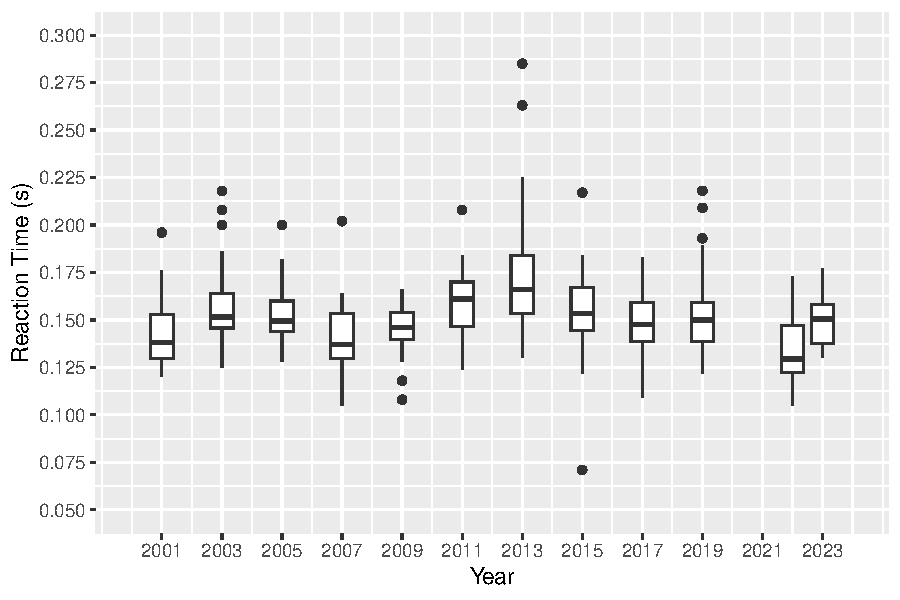
\includegraphics[width=\textwidth]{WomensBoxplot}
  \caption{The RTs from 2021 to 2023 for the women's 100 meter hurdle
  and 100 meter dash.}
  \label{fig:WomensBoxplot}
\end{figure}


\of{Currently cannot fit the gg3b to the men's and womens data}


\section{Results from Data Excluding Positive DQ RTs}
An earlier iteration of the paper fit a model but did not include RTs from
athletes who were disqualified or did not finish but still registered a reaction
time.  However, it was decided that to better estimate the left tail of the
distribution and more accurately predict the probability of a low reaction time,
those RTs should be included.  We cannot include times from athltes with a
negative reaction time, as that is a mistake of the runner for starting before
the gun is fired, and thus those times are meaningless in our objective to
determine a fair reaction time barrier.  Not all of those disqualified were
disqualified because of breaking the 0.1 reaction time barrier; there are many
reasons why an athlete may be diqualified with the most notable being a failed
drug test and lane violations.  Nonetheless, in this iteration of the analysis,
we will exclude these observations to see the effect on the probability of an
extreme reaction time.  We fit an identical model to the generalized Gamma model
presented in section 3.2 to examine differences in these types of data.

\begin{table}
  \centering
  \caption{Probabilities of observing RTs less than threshold 0.08,
  0.09, and 0.10 seconds based on the
    fitted GG GAMLSS model with both venue- and heat-level
random effects.}
  \begin{tabular}{c c c c}
   \toprule
   Data Set & Threshold 0.08 & Threshold 0.09 & Threshold 0.10  \\
   \midrule
   Without DQs & $4.93\cdot10^{-5}$ & $3.53\cdot10^{-4}$ &  $1.97\cdot10^{-3}$  \\
   With DQs & $6.84\cdot10^{-5}$ & $4.95\cdot10^{-4}$ & $2.76\cdot10^{-3}$ \\
   \bottomrule
  \end{tabular}
  \label{tab:DQSim_probability}
\end{table}

Table~\ref{tab:DQSim_probability} shows the effect of removing disqualificated
times from the analysis.  The probability of observing extreme RTs is lower when
we remove the 17 observations.

\bibliographystyle{apalike}
\bibliography{citations}


\end{document}
